\clearpage

\section{Data Wrangling and Feature Extraction}

\subsection{Exploratory Data Analysis}


\textbf{Sample Distribution}

\Cref{tab:parsed_dict} shows the structure of the dataset. A total of \note{1962} articles were collected from Smallcaps. \Cref{fig:articles_per_month} shows the time distribution over time, covering all of 2024, late 2023, and early 2025. This time window may be a limitation, as older articles could exhibit different characteristics not captured in the current dataset. \Cref{fig:document_length_distribution} depicts the document length distribution, with a mean word count of \note{462}. The dataset size and document length are sufficient for training machine learning models, particularly when using pretrained transformers such as BERT \cite{bert_paper} or FinBERT \cite{prosusai_finbert}.

\Cref{code:article_Augmentation} shows the addition of industry labels to articles using a list of stock codes retrieved from the ASX website \cite{asx_industry_labels}. These labels, along with those reported by Smallcaps, are shown in \cref{fig:sector_industry_distribution}. Most articles fall within the mining sector, indicating a sample bias. While ASX labels offer greater context, the larger amount of labels introduces sparsity, with several sectors having very few observations.

\begin{figure}[ht]
    \begin{minipage}{0.42\textwidth}
        \centering
        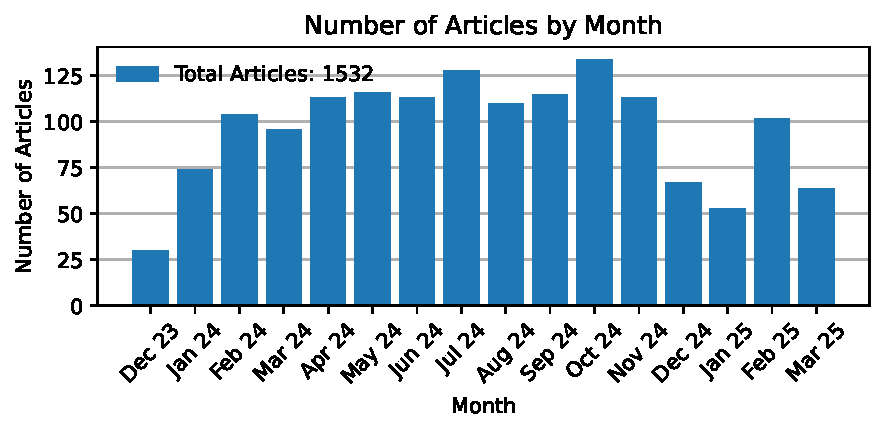
\includegraphics[width=\textwidth]{figures/articles_per_month.pdf}
        \caption{Quantity of Scraped Articles per Month}
        \label{fig:articles_per_month}
        
        \vspace{1em}
        
        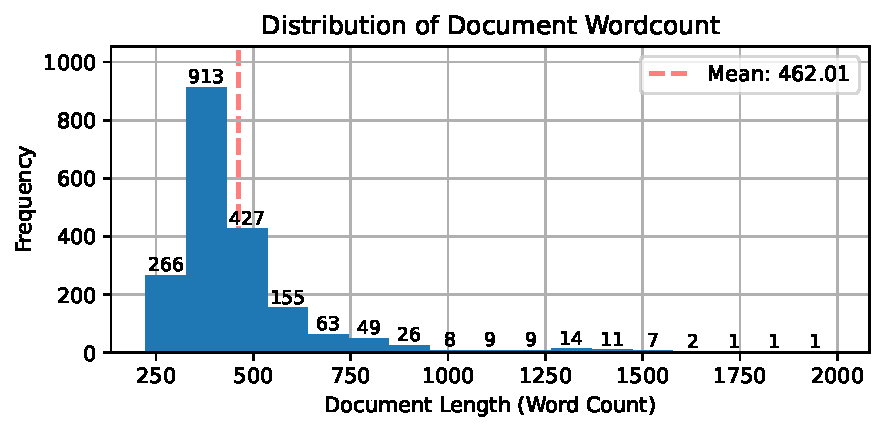
\includegraphics[width=\textwidth]{figures/document_length_distribution.pdf}
        \caption{Distribution of Document Length}
        \label{fig:document_length_distribution}
    \end{minipage}
    \hfill
    \begin{minipage}{0.55\textwidth}
        \centering
        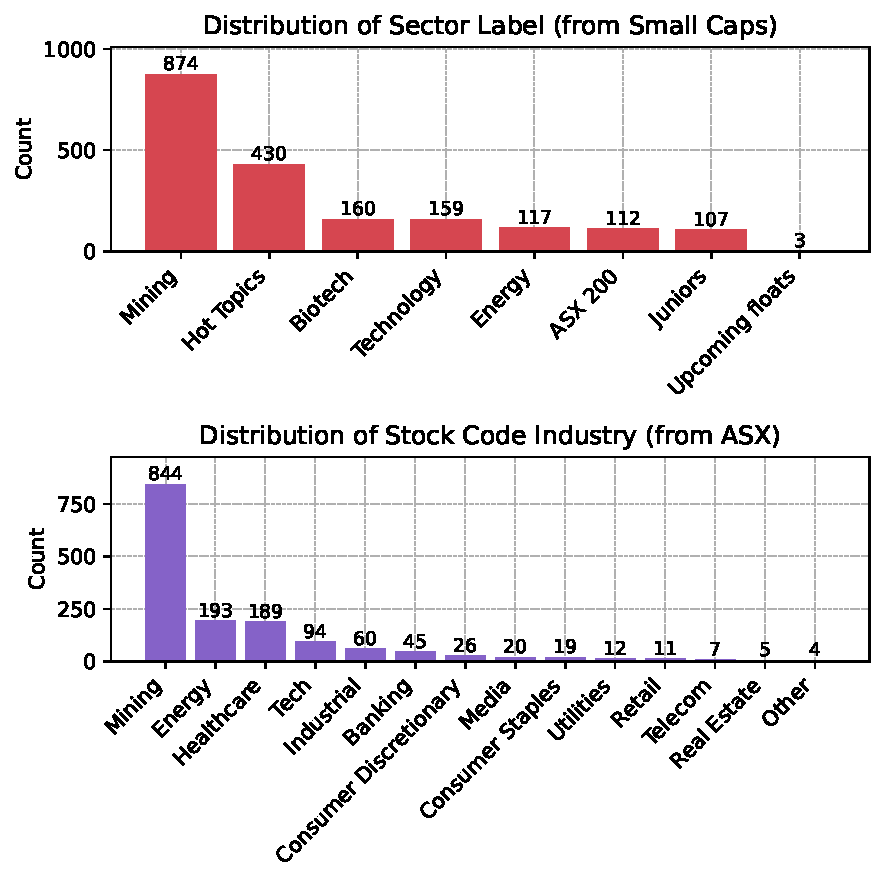
\includegraphics[width=\textwidth]{figures/sector_industry_distribution.pdf}
        \caption{Distribution of Articles by Sector, using the \textit{smallcaps} industry label and the ASX sector label \cite{asx_industry_labels}}
        \label{fig:sector_industry_distribution}
    \end{minipage}
\end{figure}

\textbf{Text Corpus}

\Cref{fig:top_words} shows the most common words in the articles, whilst removing stop words using \code{Sklearn CountVectorizer}. It can be seen that past general terms like company, project and asx, mining and resource terms are the most prevailant in the corpus, further demonstrating the mining sampling bias highlighted in \cref{fig:sector_industry_distribution}

\Cref{fig:pca} shows the PCA biplot of the TF-IDF vectorised article corpus, generated using \code{SKlearn}'s \code{PCA} and \code{TfidfVectorizer} modules. Lemmatisation was applied via \code{nltk} to reduce term dimensionality. It can be seen that even with two components, the plot shows some level of clustering by sector, suggesting that term usage differs meaningfully between them.


\begin{figure}[htbp]
    \centering
    \begin{minipage}{0.48\textwidth}
        \centering
        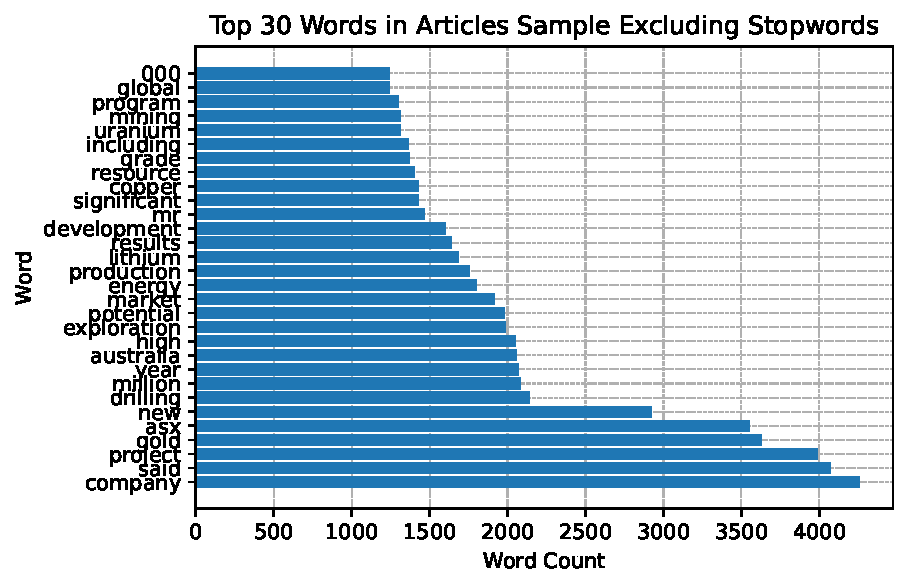
\includegraphics[width=\linewidth]{figures/top_words_in_articles.pdf}
        \caption{Frequency of the top words in the scraped articles}
        \label{fig:top_words}
    \end{minipage}\hfill
    \begin{minipage}{0.48\textwidth}
        \centering
        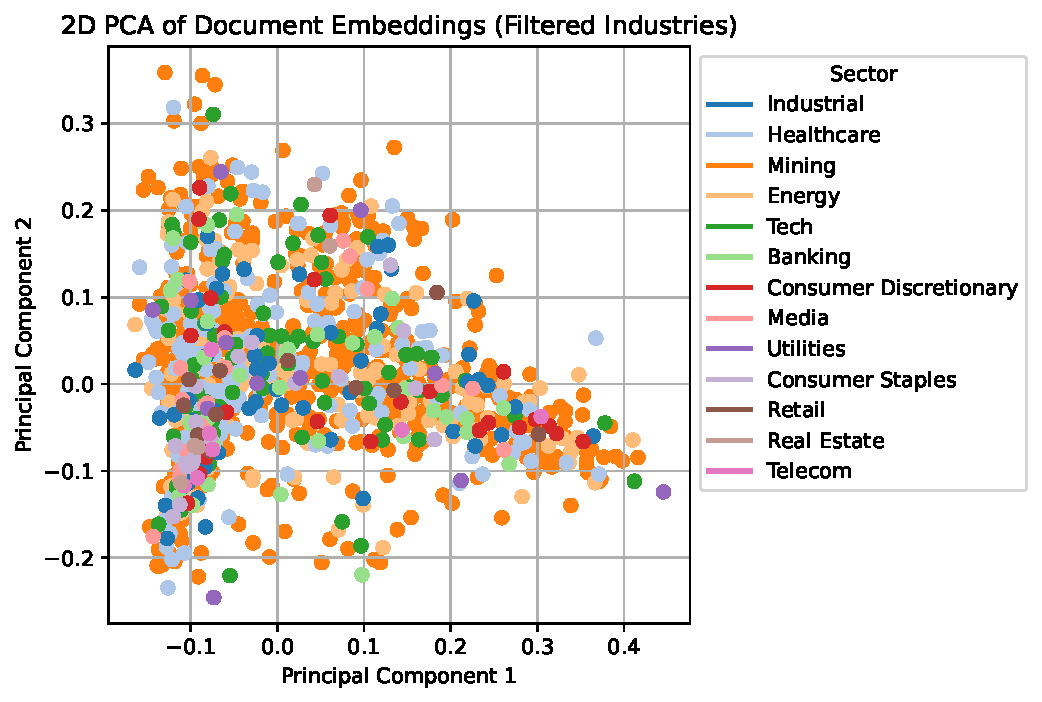
\includegraphics[width=\linewidth]{figures/pca_biplot_filtered_industries.pdf}
        \caption{Principle Component Analysis Biplot of the TF-IDF vectorised article corpus (with lemmatisation applied)}
        \label{fig:pca}
    \end{minipage}
\end{figure}








\subsection{Sentiment Analysis}

We model the sentiment of an article using the VADER (Valence Aware Dictionary and sEntiment Reasoner)\cite{vader_paper}, as this has shown to having promising results in a similar setting, as found by \cite{heiden_lstm}. Implementation of VADER can be seen in \cref{code:vader}, with the implementation inspired assisted by online article \cite{geeksforgeeks_vader}

\lstinputlisting[language=Python, caption=VADER sentiment analysis of article, label=code:vader]{../code/report_code_chunks/sentiment_vader.py}

VADER's rule-based approach relies on fixed lexicons and doesn't fully capture the context-dependent sentiment embedded in text, whereas BERT's deep contextual embeddings and bidirectional architecture captures nuanced meanings in multi-word expressions, and been pre-trained on large-scale text, including Wikipedia , BERT can recognise \note{swap up the wording here a bit}
proper nouns and entities, making it effective for
disambiguating stock names, tickers, and countries  \cite{bert_paper}. FinBERT is a domain-specific adaptation of the BERT model, fine-tuned on financial texts to accurately determine the sentiment expressed in this particular context \cite{araci_finbert}. This model was retrieved using the huggingface library \cite{prosusai_finbert}. 

While this sounds better, it relies on the data being labelled, making training on a large corupus of data unfeasible without labourious labelling. We therefore utilise the finbert-tone pretrained transformer which is the FinBERT model trained on 10,000 manually annotated documents (positive, negative, neutral) sentences from analyst reports \cite{finbert_tone_sentiment}.

\lstinputlisting[language=Python, caption=BERT sentiment analysis of articles, label=code:bert]{../code/report_code_chunks/sentiment_bert.py}

It is evident from \cref{fig:sentiment_distributions} that VADER and BERT has a high skew towards positive sentiment, potentially indicating that the authors of smallcaps are averse to publishing negative news. \Cref{fig:sentiment_heatmap} shows that other than a small amount of outliers, the BERT and VADER sentiment models are highly correlated.

\begin{figure}[h]
    \centering
    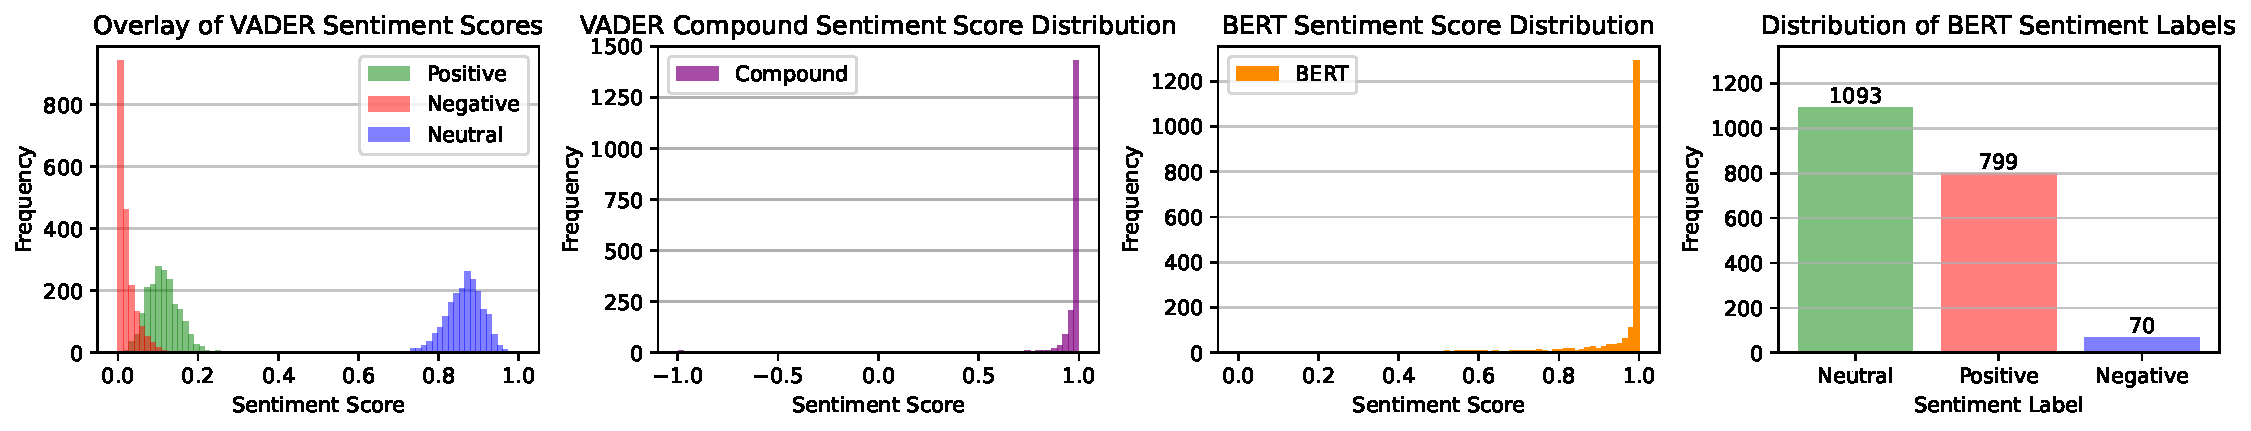
\includegraphics[width=\linewidth]{figures/sentiment_distribution.pdf} % Image filename
    \centering
    \caption{Distribution of Sentiment Labels and scores for VADER and BERT} % Caption
    \label{fig:sentiment_distributions} % Label
\end{figure}

\begin{figure}[h]
    \centering
    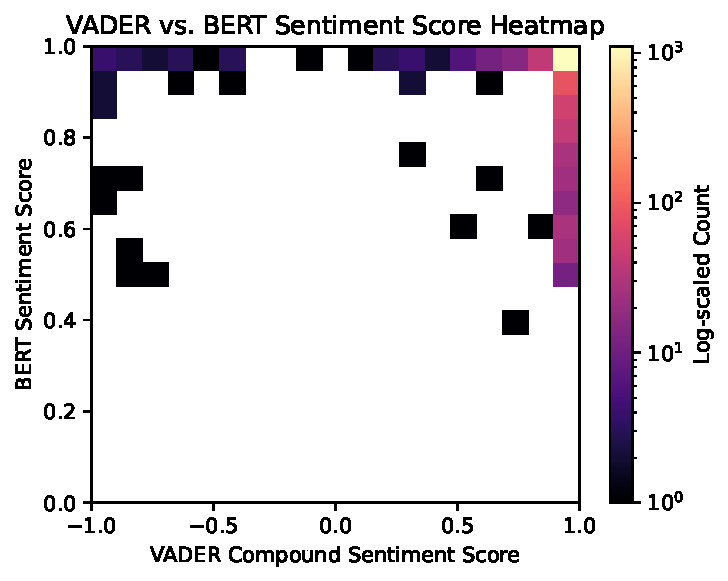
\includegraphics[height=200px]{figures/sentiment_heatmap.pdf} % Image filename
    \centering
    \caption{Heatmap Comparison of sentiment scores of VADER vs BERT} % Caption
    \label{fig:sentiment_heatmap} % Label
\end{figure}

